%% 
%% Created in 2018 by Martin Slapak
%% last update:		2021-09-21
%%
%% Based on file for NRP report LaTeX class by Vit Zyka (2008)
%% enhanced for MI-MVI (2018) and tuned for BI-PYT (2020, 2021)
%%

\documentclass[czech]{pyt-report}

\usepackage[utf8]{inputenc} 

\title{Wishlist webová aplikace}

\author{Kateřina Zusková}
\affiliation{ČVUT--FIT}
\email{zuskokat@fit.cvut.cz}

\def\file#1{{\tt#1}}

\begin{document}

\maketitle

Tento report informuje o semestrální práci vytvořené
pro předmět BI–PYT v zimním semestru B241.

%%%%%%%%%%%%%%%%%%%%%%%%%%%%%%%%%%%%%%%%%%%%%%%%%%%%%%%%%%%%%%%%%%%%%%%%%%%%%%%%
\section{Úvod}
Cílem práce je vytvořit webovou aplikaci, která by umožňovala uživatelům vytvářet, editovat a sdílet seznamy přání. Další požadovanou funkcionalitou je, aby uživatelé, se kterými je seznam sdílený, mohli jednotlivé položky na seznamu tzv. rezervovat. Všichni uživatelé, se kterými je seznam sdílený, vidí, které položky jsou rezervované. Majitel seznamu nevidí, které položky jsou rezervované. Další funkcionalitou je archivace a mazání seznamů - v archivovaném seznamu nelze manipulovat s položkami a vidí jej pouze majitel. Majitel seznamu také může položky tzv. přijmout. Všichni uživatelé, se kterými je seznam sdílený, vidí, které položky jsou přijaté, a nemohou je rezervovat.
\\
\\
Aplikace je spuštěná na: \url{https://wishlist.mag.wiki/}

%%%%%%%%%%%%%%%%%%%%%%%%%%%%%%%%%%%%%%%%%%%%%%%%%%%%%%%%%%%%%%%%%%%%%%%%%%%%%%%%
\section{HTMX}
Jelikož jsem neměla zkušenosti s vývojem dynamických webových stránek a nikdy jsem nepoužívala java-script ani react, rozhodla jsem se, že pro mě bude jednodušší použít HTMX. Díky HTMX je také načítání změn na webové stránce rychlejší - místo načítání celé stránky načte pouze její část.

%%%%%%%%%%%%%%%%%%%%%%%%%%%%%%%%%%%%%%%%%%%%%%%%%%%%%%%%%%%%%%%%%%%%%%%%%%%%%%%%
\section{UIkit}
Pro tvorbu front-endu jsem zvolila front-end frame-work UIkit. To sice limituje design webové stránky, ale značně mi to usnadnilo jeho vývoj. Prvotní návrh designu (ten se v průběhu implementace trochu změnil, viz obrázky \ref{fig:register} \ref{fig:login} \ref{fig:wishlist} \ref{fig:shared}) byl jednodušší, rychlejší a pomocí UIkitu se dalo všeho s mírnými kompromisy dosáhnout.

\begin{figure}[h]
  \centering\leavevmode
  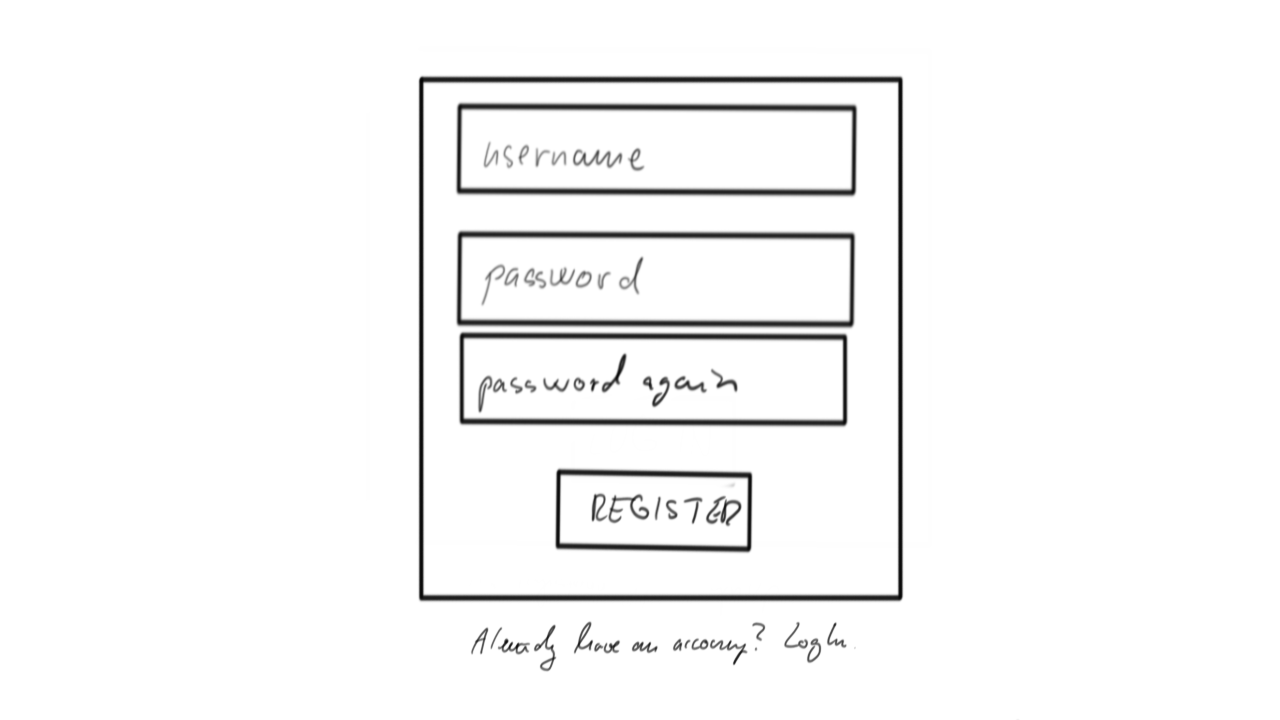
\includegraphics[width=0.8\linewidth]{img/register_page.png}\vskip-0.5cm
  \caption{návrh registrační stránky}
  \label{fig:register}
\end{figure}
\begin{figure}[h]
  \centering\leavevmode
  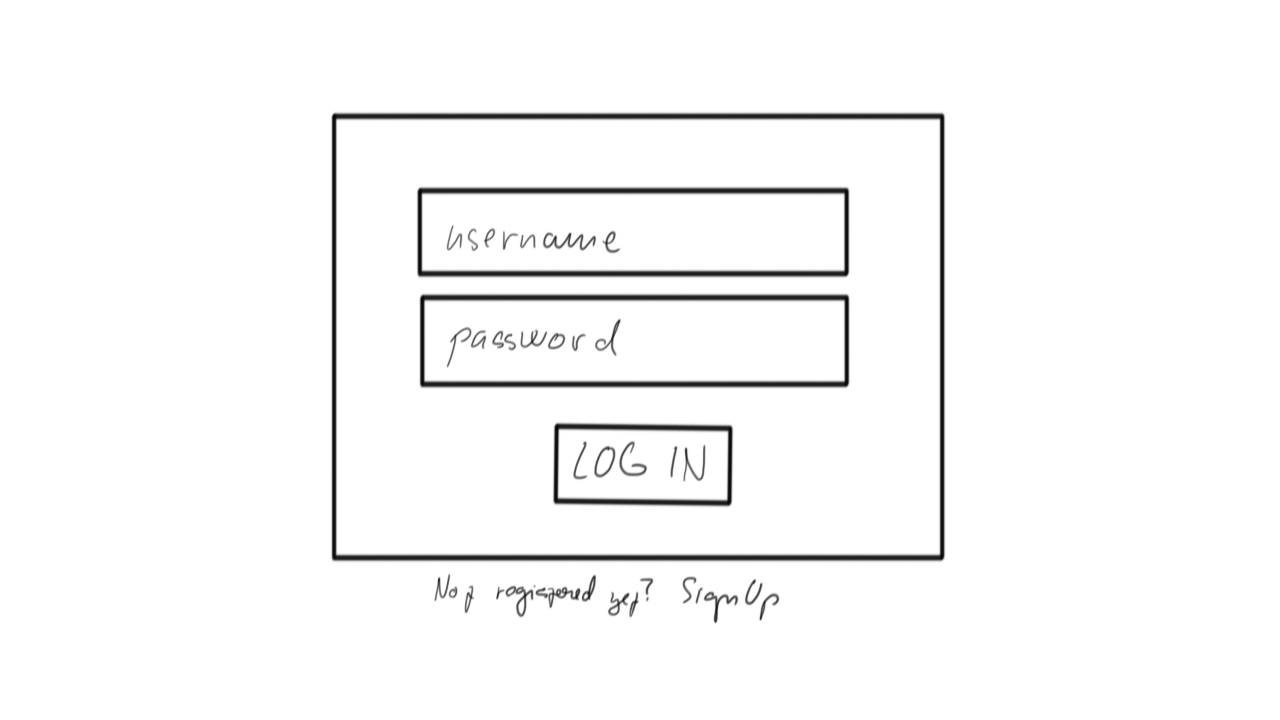
\includegraphics[width=0.8\linewidth]{img/login_page.png}\vskip-0.5cm
  \caption{návrh přihlašovací stránky}
  \label{fig:login}
\end{figure}
\begin{figure}[h]
  \centering\leavevmode
  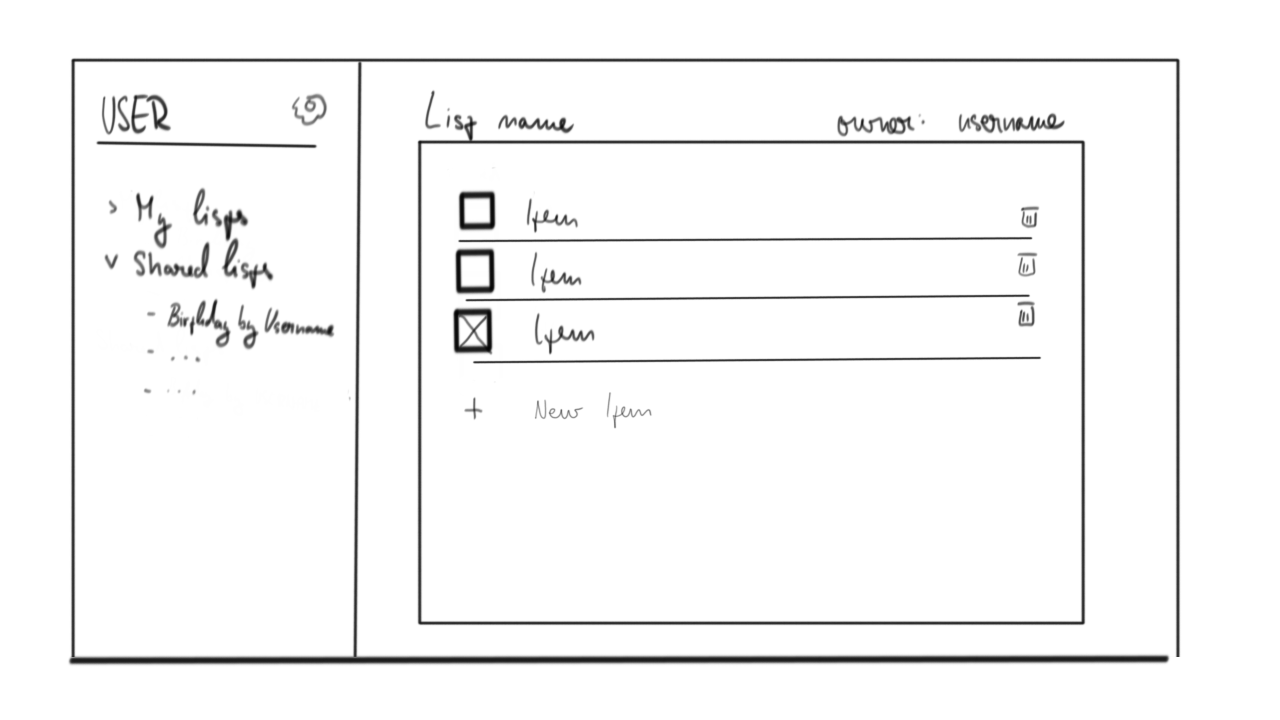
\includegraphics[width=0.8\linewidth]{img/wishlist_page.png}\vskip-0.5cm
  \caption{návrh stránky s vlastním seznamem}
  \label{fig:wishlist}
\end{figure}
\begin{figure}[h]
  \centering\leavevmode
  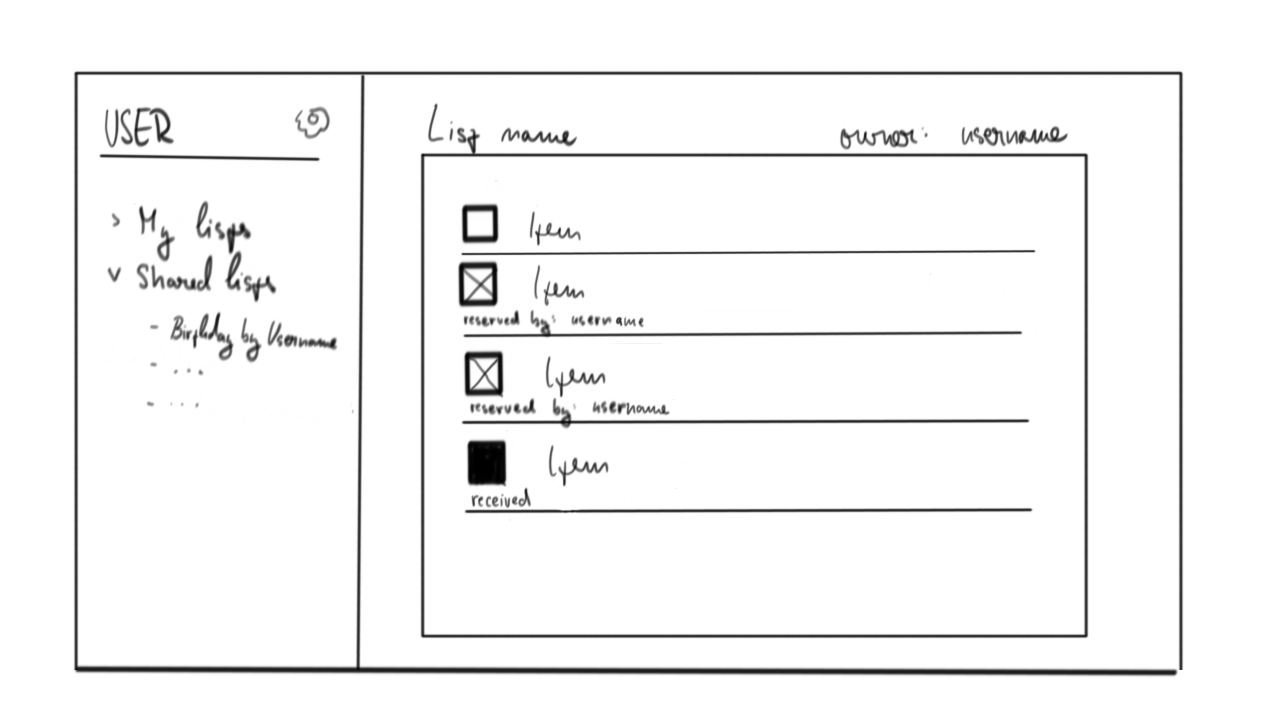
\includegraphics[width=0.8\linewidth]{img/shared_page.png}\vskip-0.5cm
  \caption{návrh stránky s nasdíleným seznamem}
  \label{fig:shared}
\end{figure}

\clearpage
%%%%%%%%%%%%%%%%%%%%%%%%%%%%%%%%%%%%%%%%%%%%%%%%%%%%%%%%%%%%%%%%%%%%%%%%%%%%%%%%
\section{Databáze}
Pro správné fungování aplikace je potřebná databáze, která bude ukládat inforamce o uživatelích, seznamech a položkách. Pro implementaci databáze jsem zvolila sqlite, která pro projekt této velikosti stačí. Pro ORM jsem zvolila knihovnu SQLAlchemy. Databáze obsahuje entity User, Wishlist a Item, viz obrázek \ref{fig:db}. Důležitá je také tabulka, která obsahuje informace o tom, se kterými uživateli jsou jednotlivé seznamy nasdílené. Databáze nemá naimplementované povinné relace, nicméně API takovou situaci neumožňuje.

\begin{figure}[h]
  \centering\leavevmode
  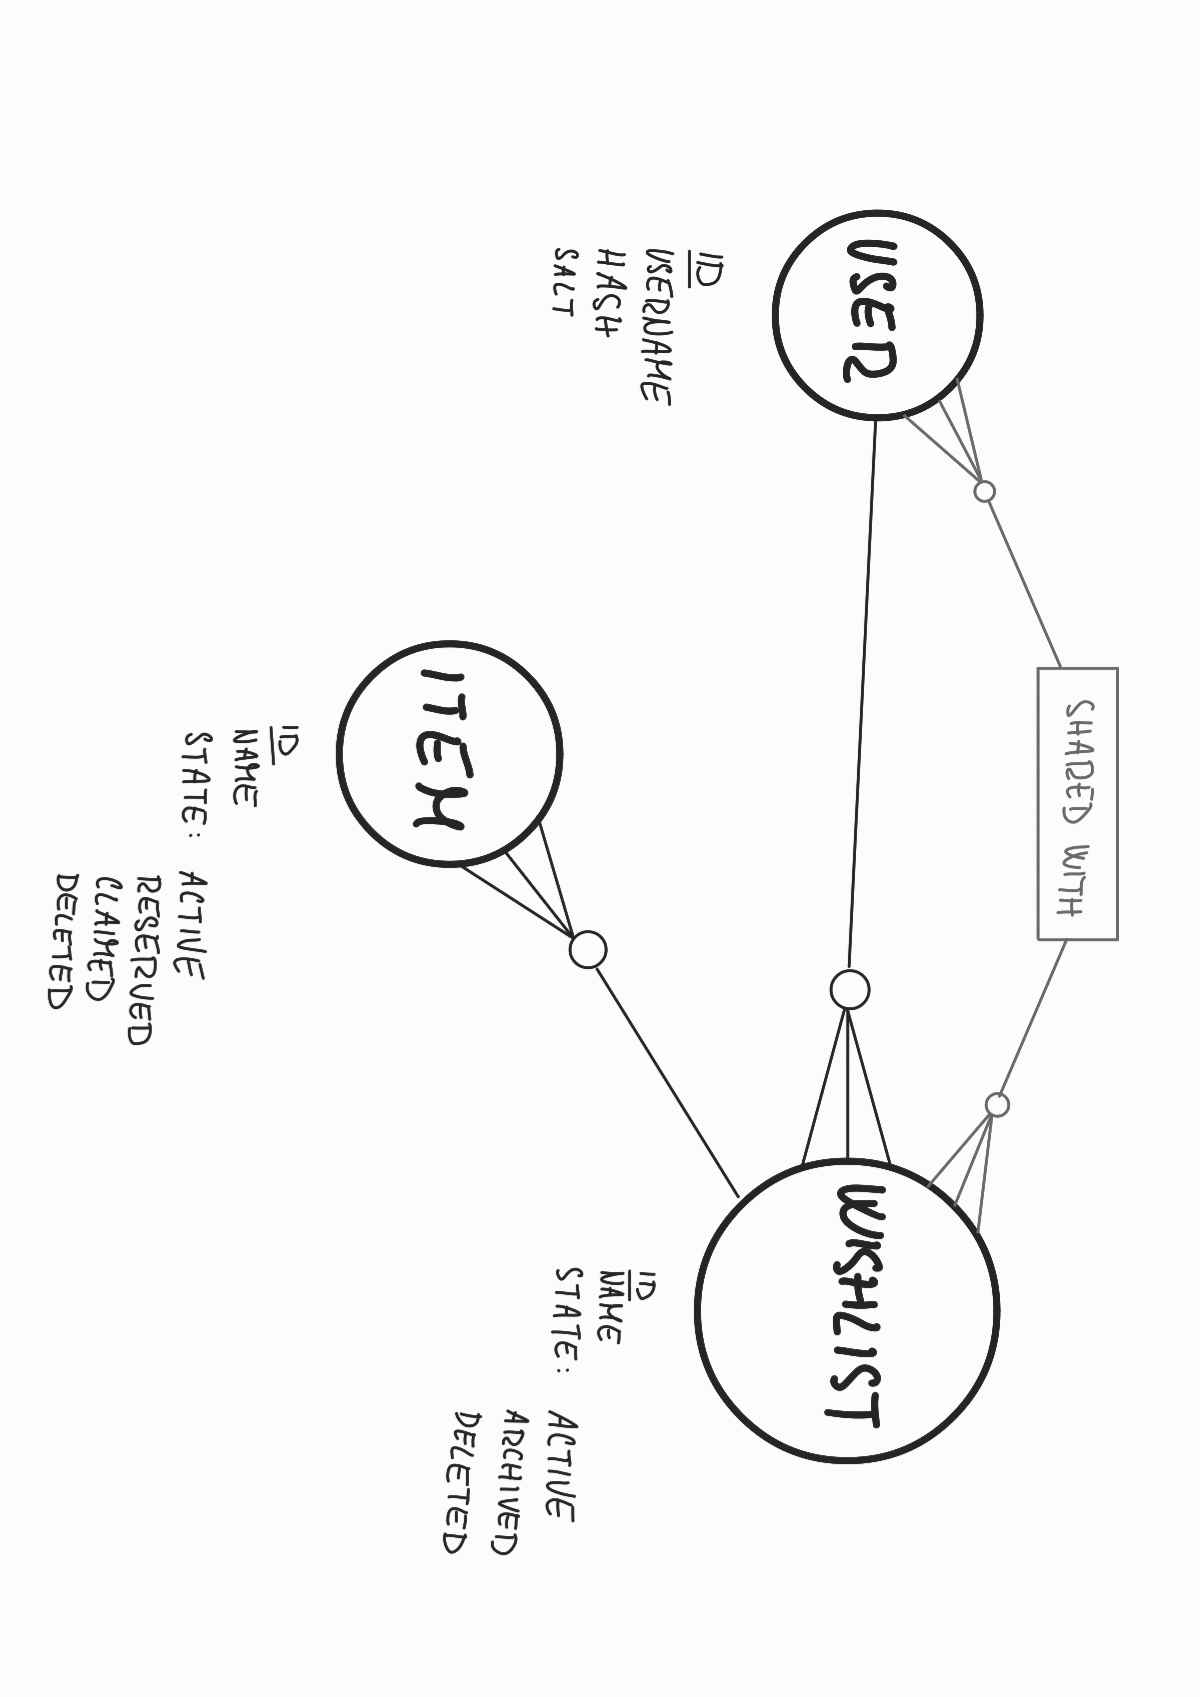
\includegraphics[angle=90,width=1\linewidth]{img/database.jpg}\vskip-0.5cm
  \caption{zjednoduššené schéma databáze}
  \label{fig:db}
\end{figure}

%%%%%%%%%%%%%%%%%%%%%%%%%%%%%%%%%%%%%%%%%%%%%%%%%%%%%%%%%%%%%%%%%%%%%%%%%%%%%%%%
\section{Autorizace}
Pro správné fungování aplikace je podstatná registrace a autorizace uživatelů. Zvolila jsem knihovnu flask-login, která celý proces zjednodušuje. Tato knihovna usnadňuje přesměrování uživatele, kontrolu, zda je uživatel přihlášený v situacích, které to vyžadují a nastavuje proměnnou current\textunderscore user, což značně usnadňuje development.

%%%%%%%%%%%%%%%%%%%%%%%%%%%%%%%%%%%%%%%%%%%%%%%%%%%%%%%%%%%%%%%%%%%%%%%%%%%%%%%%
\section{Zabezpečení}
Webové aplikace jsou náchylné k útokům zvenčí. Uživatelská hesla jsou zabezpečená pomocí hash with salt metody, kterou zprostředkovává knihovna werkzeug. SQL-injections ošetřuje knihovna SQLAlchemy a XSS útoky jsou ošetřené díky flask templatingu (pomocí knihovny jinja, kterou flask používá). Program také myslí na to, aby uživatelé nemohli manipulovat se seznamy, které nejsou jejich a podobně (například uživatel nemůže přidat položku na seznam, který není jeho).


%%%%%%%%%%%%%%%%%%%%%%%%%%%%%%%%%%%%%%%%%%%%%%%%%%%%%%%%%%%%%%%%%%%%%%%%%%%%%%%%
% --- ZAVER
\section{Závěr}
Díky této práci lépe rozumím fungování webových aplikací a umím vytvářet dynamické webové stránky. S výsledkem jsem spokojená, aplikace funguje a věřím, že bude užitečná. Do budoucnosti je možná spousta vylepšíní, například: 
\begin{itemize}
  \item sdílení pomocí odkazu
  \item možnost změny pořadí položek v seznamu
  \item zobrazení jména uživatele, který rezervoval položku
  \item automatické mazání převzatých položek po nějaké době
  \item možnost smazání uživatelského účtu
\end{itemize}
Nejsem zcela spokojená s UI designem webové stránky. Raději jsem se soustředila na ostatní funkcionality a implementaci v pythonu a výsledek je tak spíše proof of concept, nicméně design je podle mě zcela dostačující. Určitě by ale do budoucnosti zasloužil změny, aby byl uživatelsky příjemnější.
\\
Příště by bylo lepší věnovat více času naplánování projektu a funkcionalit hned na začátku. Při tvorbě této práce jsem přidávala hodně věcí za běhu a ne vždy to bylo optimální.
\\
Vzhledem k tomu, že se pro mě jednalo o první seznámení s webovou aplikací, považuji výsledek za úspěšný.

%%%%%%%%%%%%%%%%%%%%%%%%%%%%%%%%%%%%%%%%%%%%%%%%%%%%%%%%%%%%%%%%%%%%%%%%%%%%%%%%
% --- Bibliography
\nocite{pyt_doc}
\nocite{flask_doc}
\nocite{flask_sql_alch}
\nocite{sql_alch}
\nocite{flask_login}
\nocite{login_readme}
\nocite{werk}
\nocite{waitress}
\nocite{uikit}
\nocite{htmx}
\nocite{lukas}
%\bibliographystyle{plain-cz-online}
\bibliography{reference}

\end{document}
